\documentclass[10pt]{article}
\usepackage{../pplmanual}
\NeedsTeXFormat{LaTeX2e}
\typeout{^^J^^J
Parallel Programming Laboratory^^J
Manual Style^^J
Written by Milind A. Bhandarkar, 12/00^^J}

%%% Make it possible for both ps and pdf to be generated
\newif\ifpdf
\ifx\pdfoutput\undefined
  \pdffalse
\else
  \pdfoutput=1
  \pdftrue
\fi

\ifpdf
  \pdfcompresslevel=9
\fi

%%% Imported from fullpage.sty, since it is not always available
\topmargin 0pt
\advance \topmargin by -\headheight
\advance \topmargin by -\headsep

\textheight 8.9in

\oddsidemargin 0pt
\evensidemargin \oddsidemargin
\marginparwidth 1.0in

\textwidth 6.5in
%%% end import from fullpage

%%% Commonly Needed packages
\usepackage{graphicx,color,calc}
\usepackage{makeidx}
\usepackage{alltt}

%%% Commands for uniform looks of C++, Charm++, and Projections
\newcommand{\CC}{C\kern -0.0em\raise 0.5ex\hbox{\normalsize++}}
\newcommand{\emCC}{C\kern -0.0em\raise 0.4ex\hbox{\normalsize\em++}}
\newcommand{\charmpp}{\sc Charm++}
\newcommand{\projections}{\sc Projections}
\newcommand{\converse}{\sc Converse}
\newcommand{\ampi}{\sc AMPI}

%%% Commands to produce margin symbols
\newcommand{\new}{\marginpar{\fbox{\bf$\mathcal{NEW}$}}}
\newcommand{\important}{\marginpar{\fbox{\bf\Huge !}}}
\newcommand{\experimental}{\marginpar{\fbox{\bf\Huge $\beta$}}}

%%% Commands for manual elements
\newcommand{\zap}[1]{ }
\newcommand{\function}[1]{{\noindent{\textsf{#1}}\\}}
\newcommand{\cmd}[1]{{\noindent{\textsf{#1}}\\}}
\newcommand{\args}[1]{\hspace*{2em}{\texttt{#1}}\\}
\newcommand{\param}[1]{{\texttt{#1}}}
\newcommand{\kw}[1]{{\textsf{#1}}}
\newcommand{\uw}[1]{{\textsl{#1}}}
\newcommand{\desc}[1]{\indent{#1}}

%%% Commands needed for Maketitle
\newcommand{\@version}{}
\newcommand{\@credits}{}
\newcommand{\version}[1]{\renewcommand{\@version}{#1}}
\newcommand{\credits}[1]{\renewcommand{\@credits}{#1}}

%%% Print the License Page
\newcommand{\@license}{%
 \begin{center}
   {University of Illinois}\\
   {\charmpp/\converse\ Parallel Programming System Software}\\
   {Non-Exclusive, Non-Commercial Use License}\\
 \end{center}
 \rule{\textwidth}{1pt}
{\tiny
Upon execution of this Agreement by the party identified below (``Licensee''),
The Board of Trustees of the University of Illinois  (``Illinois''), on behalf
of The Parallel Programming Laboratory (``PPL'') in the Department of Computer
Science, will provide the \charmpp/\converse\ Parallel Programming System
software (``\charmpp'') in Binary Code and/or Source Code form (``Software'')
to Licensee, subject to the following terms and conditions. For purposes of
this Agreement, Binary Code is the compiled code, which is ready to run on
Licensee's computer.  Source code consists of a set of files which contain the
actual program commands that are compiled to form the Binary Code.

\begin{enumerate}
  \item
    The Software is intellectual property owned by Illinois, and all right,
title and interest, including copyright, remain with Illinois.  Illinois
grants, and Licensee hereby accepts, a restricted, non-exclusive,
non-transferable license to use the Software for academic, research and
internal business purposes only, e.g. not for commercial use (see Clause 7
below), without a fee.

  \item 
    Licensee may, at its own expense, create and freely distribute
complimentary works that interoperate with the Software, directing others to
the PPL server (\texttt{http://charm.cs.uiuc.edu}) to license and obtain the
Software itself. Licensee may, at its own expense, modify the Software to make
derivative works.  Except as explicitly provided below, this License shall
apply to any derivative work as it does to the original Software distributed by
Illinois.  Any derivative work should be clearly marked and renamed to notify
users that it is a modified version and not the original Software distributed
by Illinois.  Licensee agrees to reproduce the copyright notice and other
proprietary markings on any derivative work and to include in the documentation
of such work the acknowledgement:

\begin{quote}
``This software includes code developed by the Parallel Programming Laboratory
in the Department of Computer Science at the University of Illinois at
Urbana-Champaign.''
\end{quote}

Licensee may redistribute without restriction works with up to 1/2 of their
non-comment source code derived from at most 1/10 of the non-comment source
code developed by Illinois and contained in the Software, provided that the
above directions for notice and acknowledgement are observed.  Any other
distribution of the Software or any derivative work requires a separate license
with Illinois.  Licensee may contact Illinois (\texttt{kale@cs.uiuc.edu}) to
negotiate an appropriate license for such distribution.

  \item
    Except as expressly set forth in this Agreement, THIS SOFTWARE IS PROVIDED
``AS IS'' AND ILLINOIS MAKES NO REPRESENTATIONS AND EXTENDS NO WARRANTIES OF
ANY KIND, EITHER EXPRESS OR IMPLIED, INCLUDING BUT NOT LIMITED TO WARRANTIES OR
MERCHANTABILITY OR FITNESS FOR A PARTICULAR PURPOSE, OR THAT THE USE OF THE
SOFTWARE WILL NOT INFRINGE ANY PATENT, TRADEMARK, OR OTHER RIGHTS.  LICENSEE
ASSUMES THE ENTIRE RISK AS TO THE RESULTS AND PERFORMANCE OF THE SOFTWARE
AND/OR ASSOCIATED MATERIALS.  LICENSEE AGREES THAT UNIVERSITY SHALL NOT BE HELD
LIABLE FOR ANY DIRECT, INDIRECT, CONSEQUENTIAL, OR INCIDENTAL DAMAGES WITH
RESPECT TO ANY CLAIM BY LICENSEE OR ANY THIRD PARTY ON ACCOUNT OF OR ARISING
FROM THIS AGREEMENT OR USE OF THE SOFTWARE AND/OR ASSOCIATED MATERIALS.

  \item 
    Licensee understands the Software is proprietary to Illinois. Licensee
agrees to take all reasonable steps to insure that the Software is  protected
and secured from unauthorized disclosure, use, or release and  will treat it
with at least the same level of care as Licensee would use to  protect and
secure its own proprietary computer programs and/or information, but using no
less than a reasonable standard of care.  Licensee agrees to provide the
Software only to any other person or entity who has registered with Illinois.
If licensee is not registering as an individual but as an institution or
corporation each member of the institution or corporation who has access to or
uses Software must agree to and abide by the terms of this license. If Licensee
becomes aware of any unauthorized licensing, copying or use of the Software,
Licensee shall promptly notify Illinois in writing. Licensee expressly agrees
to use the Software only in the manner and for the specific uses authorized in
this Agreement.

  \item
    By using or copying this Software, Licensee agrees to abide by the
copyright law and all other applicable laws of the U.S. including, but not
limited to, export control laws and the terms of this license. Illinois  shall
have the right to terminate this license immediately by written  notice upon
Licensee's breach of, or non-compliance with, any terms of the license.
Licensee may be held legally responsible for any  copyright infringement that
is caused or encouraged by its failure to  abide by the terms of this license.
Upon termination, Licensee agrees to  destroy all copies of the Software in its
possession and to verify such  destruction in writing.

  \item
  The user agrees that any reports or published results obtained with  the
Software will acknowledge its use by the appropriate citation as  follows:

\begin{quote}
``\charmpp/\converse\ was developed by the Parallel Programming Laboratory in
the Department of Computer Science at the University of  Illinois at
Urbana-Champaign.''
\end{quote}

Any published work which utilizes \charmpp\ shall include the following
reference:

\begin{quote}
``L. V. Kale and S. Krishnan. \charmpp: Parallel Programming with Message-Driven
Objects. In 'Parallel Programming using \CC' (Eds. Gregory V. Wilson and Paul
Lu), pp 175-213, MIT Press, 1996.''
\end{quote}

Any published work which utilizes \converse\ shall include the following
reference:

\begin{quote}
``L. V. Kale, Milind Bhandarkar, Narain Jagathesan, Sanjeev Krishnan and Joshua
Yelon. \converse: An Interoperable Framework for Parallel Programming.
Proceedings of the 10th International Parallel Processing Symposium, pp
212-217, April 1996.''
\end{quote}

Electronic documents will include a direct link to the official \charmpp\ page
at \texttt{http://charm.cs.uiuc.edu/}

  \item
    Commercial use of the Software, or derivative works based thereon,
REQUIRES A COMMERCIAL LICENSE.  Should Licensee wish to make commercial use of
the Software, Licensee will contact Illinois (kale@cs.uiuc.edu) to negotiate an
appropriate license for such use. Commercial use includes: 

    \begin{enumerate}
      \item
	integration of all or part of the Software into a product for sale,
lease or license by or on behalf of Licensee to third parties, or 

      \item
	distribution of the Software to third parties that need it to
commercialize product sold or licensed by or on behalf of Licensee.
    \end{enumerate}

  \item
    Government Rights. Because substantial governmental funds have been  used
in the development of \charmpp/\converse, any possession, use or sublicense of
the Software by or to the United States government shall be subject to such
required restrictions.

  \item
    \charmpp/\converse\ is being distributed as a research and teaching tool
and as such, PPL encourages contributions from users of the code that might, at
Illinois' sole discretion, be used or incorporated to make the basic  operating
framework of the Software a more stable, flexible, and/or useful  product.
Licensees who contribute their code to become an internal  portion of the
Software agree that such code may be distributed by  Illinois under the terms
of this License and may be required to sign an  ``Agreement Regarding
Contributory Code for \charmpp/\converse\ Software'' before Illinois  can
accept it (contact \texttt{kale@cs.uiuc.edu} for a copy).
\end{enumerate}

UNDERSTOOD AND AGREED.

Contact Information:

The best contact path for licensing issues is by e-mail to
\texttt{kale@cs.uiuc.edu} or send correspondence to:

\begin{quote}
Prof. L. V. Kale\\
Dept. of Computer Science\\
University of Illinois\\
1304 W. Springfield Ave\\
Urbana, Illinois 61801 USA\\
FAX: (217) 333-3501
\end{quote}
}%tiny
 \newpage
}% end of license

\renewcommand{\maketitle}{\begin{titlepage}%
 \begin{flushright}
   {\Large
     Parallel Programming Laboratory\\
     University of Illinois at Urbana-Champaign\\
   }
 \end{flushright}
 \rule{\textwidth}{3pt}
 \vspace{\fill}
 \begin{flushright}
   \textsf{\Huge \@title \\}
 \end{flushright}
 \vspace{\fill}
 \@credits \\
 \rule{\textwidth}{3pt}
 \begin{flushright}
   {\large Version \@version}
 \end{flushright}
 \end{titlepage}
 \@license

 \tableofcontents
 \newpage
}% maketitle



\makeindex

\title{\charmpp\\ NetFEM\\ Manual}
\version{1.0}
\credits{
The initial version of \charmpp{} NetFEM Framework was developed
by Orion Lawlor in 2001.
}

\begin{document}

\maketitle

\section{Introduction}

NetFEM was built to provide an easy way to visualize
the current state of a finite-element simulation, or any 
parallel program that computes on an unstructured mesh.
NetFEM is designed to require very little effort to add
to a program, and connects to the running program over
the network via the network protocol CCS (Converse Client/Server).


\section{Compiling and Installing}

NetFEM is part of \charmpp{}, so it can be downloaded
as part of charm.  To build NetFEM, just build FEM normally,
or else do a make in charm/net-linux/tmp/libs/ck-libs/netfem/.

To link with NetFEM, add \kw{-module netfem} to your
program's link line.  Note that you do {\em not} need to use
the FEM framework to use NetFEM.

The netfem header file for C is called ``netfem.h'',
the header for fortran is called `netfemf.h'.
A simple example NetFEM program is in 
  charm/pgms/charm++/fem/simple2D/.
A more complicated example is in
  charm/pgms/charm++/fem/crack2D/.


\section{Running NetFEM Online}

Once you have a NetFEM program, you can run it and view 
the results online by starting the program with CCS enabled:

\begin{verbatim}
   foo.bar.edu>  ./charmrun ./myprogram +p2 ++server ++server-port 1234
\end{verbatim}

``++server-port'' controls the TCP port number to use for CCS---here,
we use 1234.  Currently, NetFEM only works with one chunk per
processor---that is, the -vp option cannot be used.

To view the results online, you then start the NetFEM client, 
which can be downloaded for Linux or Windows from 

\begin{verbatim}
http://charm.cs.uiuc.edu/research/fem/netfem/
\end{verbatim}

Enter the name of the machine running charmrun and
the TCP port number into the NetFEM client---for example, 
you might run:

\begin{verbatim}
  netfem foo.bar.edu:1234
\end{verbatim}

The NetFEM client will then connect to the program,
download the most recent mesh registered with 
\kw{NetFEM\_POINTAT}, and display it.
At any time, you can press the ``update'' button 
to reload the latest mesh.


\section{Running NetFEM Offline}

Rather than using CCS as above, you can register your meshes
using \kw{NetFEM\_WRITE}, which makes the server write out 
binary output dump files.  For example, to view timestep 10,
which is written to the ``NetFEM/10/`` directory, you'd 
run the client program as:

\begin{verbatim}
  netfem NetFEM/10
\end{verbatim}

In offline mode, the ``update'' button fetches the next
extant timestep directory.

\section{NetFEM with other Visualization Tools}

You can use a provided converter program to convert the offline NetFEM files into an XML format compatible with the powerful offline visualization tool ParaView(\url{http://paraview.org}). The converter is located in .../charm/src/libs/ck-libs/netfem/ParaviewConverter/. Build the converter by simply issuing a ``make'' command in that directory(assuming NetFEM already has been built).



Run the converter from the parent directory of the "NetFEM" directory to be converted. The converter will generate a directory called ``ParaViewData'', which contains subdirectories for each timestep, along with a ``timestep''directory for index files for each timestep. All files in the ParaViewData directory can be opened by ParaView. To open all chunks for a given timestep, open the desired timestep file in ``ParaViewData/timesteps''. Also, individual partition files can also be opened from ``ParaViewData / $<$timestep$>$ / $<$partition\_num$>$''.



\section{Interface Basics}

You publish your data via NetFEM by making a series of
calls to describe the current state of your data.  
There are only 6 possible calls you can make.

\kw{NetFEM\_Begin} is the first routine you call.
\kw{NetFEM\_End} is the last routine to call.  These
two calls bracket all the other NetFEM calls.

\kw{NetFEM\_Nodes} describes the properties of the
nodes, or vertices of the domain.  \kw{NetFEM\_Elements}
describes the properties of your elements (triangles,
tetrahedra, etc.).  After making one of these calls,
you list the different data arrays associated with your 
nodes or elements by making calls to \kw{NetFEM\_Scalar} 
or \kw{NetFEM\_Vector}.

For example, a typical finite element simulation might
have a scalar mass and vector position, velocity, and net force
associated with each node; and have a scalar stress value
associated with each element.  The sequence of NetFEM calls
this application would make would be:

\begin{verbatim}
  NetFEM_Begin
    NetFEM_Nodes -- lists position of each node
      NetFEM_Vector -- lists velocity of each node
      NetFEM_Vector -- lists net force on each node
      NetFEM_Scalar -- lists mass of each node
    
    NetFEM_Elements -- lists the nodes of each element
      NetFEM_Scalar -- lists the stress of each element
  
  NetFEM_End
\end{verbatim}

\begin{figure}[h]
\begin{center}
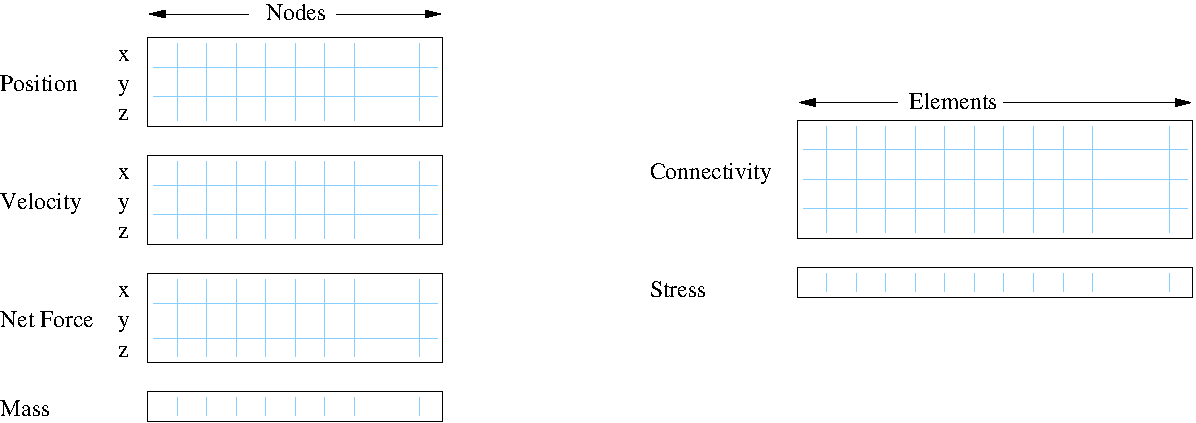
\includegraphics[width=5in]{fig/example}
\end{center}
\caption{These arrays, typical of a finite element analysis
program, might be passed into NetFEM.}
\label{fig:example}
\end{figure}


\section{Simple Interface}
The details of how to make each call are:

\prototype{NetFEM\_Begin}
\function{NetFEM NetFEM\_Begin(int source, int step, int dim, int flavor);}
\function{integer function NetFEM\_Begin(source,step,dim,flavor)}
  \args{integer, intent(in)  :: source,step,dim,flavor}

Begins describing a single piece of a mesh.  Returns a handle
that is used for each subsequent call until \kw{NetFEM\_End}.  
This call, like all NetFEM calls, is collective---every processor 
should make the same calls in the same order.

\uw{source} identifies the piece of the mesh---use FEM\_My\_partition
or CkMyPe.

\uw{step} identifies which version of the mesh this is---for example,
you might use the timestep number.  This is only used to identify the
mesh in the client.

\uw{dim} is the number of spatial dimensions.  For example, in a 2D
computation, you'd pass dim==2; in a 3D computation, dim==3.
The client currently only supports 2D or 3D computations.

\uw{flavor} specifies what to do with the data.  This can
take the value \kw{NetFEM\_POINTAT}, which is used in online visualization,
and specifies that NetFEM should only keep a pointer to your data 
rather than copy it out of your arrays.  Or it can take the value
\kw{NetFEM\_WRITE}, which writes out the data to files named
``NetFEM/\uw{step}/\uw{source}.dat'' for offline visualization. 


\prototype{NetFEM\_End}
\function{void NetFEM\_End(NetFEM n);}
\function{subroutine NetFEM\_End(n)}
  \args{integer, intent(in)  :: n}

Finishes describing a single piece of a mesh, which 
then makes the mesh available for display.


\prototype{NetFEM\_Nodes}
\function{void NetFEM\_Nodes(NetFEM n,int nNodes,const double *loc,const char *name);}
\function{subroutine NetFEM\_Nodes(n,nNodes,loc,name)}
  \args{integer, intent(in)  :: n, nNodes}
  \args{double precision, intent(in)  :: loc(dim,nNodes) }
  \args{character*(*), intent(in)  :: name}

Describes the nodes in this piece of the mesh.

\uw{n} is the NetFEM handle obtained from \kw{NetFEM\_Begin}.

\uw{nNodes} is the number of nodes listed here.

\uw{loc} is the location of each node.  This must be double-precision
array, laid out with the same number of dimentions as passed to 
\kw{NetFEM\_Begin}.  For example, in C the location of a 2D
node $n$ is stored in loc[2*n+0] (x coordinate) and loc[2*n+1]
(y coordinate).  In Fortran, location of a node $n$ is stored 
in loc(:,n).

\uw{name} is a human-readable name for the node locations
to display in the client.  We recommend also including the location
units here, for example "Position (m)".


\prototype{NetFEM\_Elements}
\function{void NetFEM\_Elements(NetFEM n,int nElements,int nodePerEl,const int *conn,const char *name);}
\function{subroutine NetFEM\_Elements(n,nElements,nodePerEl,conn,name)}
  \args{integer, intent(in)  :: n, nElements, nodePerEl}
  \args{integer, intent(in)  :: conn(nodePerEl,nElements) }
  \args{character*(*), intent(in)  :: name}

Describes the elements in this piece of the mesh.
Unlike \kw{NetFEM\_Nodes}, this call can be repeated
if there are different types of elements (For example, 
some meshes contain a mix of triangles and quadrilaterals).

\uw{n} is the NetFEM handle obtained from \kw{NetFEM\_Begin}.

\uw{nElements} is the number of elements listed here.

\uw{nodePerEl} is the number of nodes for each element.
For example, a triangle has 3 nodes per element; while 
tetrahedra have 4.

\uw{conn} gives the index of each element's nodes.  Note
that when called from C, the first node is listed in 
\uw{conn} as 0 (0-based node indexing), and element $e$'s
first node is stored in conn[e*nodePerEl+0].
When called from Fortran, the first node is listed as 1 
(1-based node indexing), and element $e$'s first node is
stored in conn(1,e) or conn((e-1)*nodePerEl+1).

\uw{name} is a human-readable name for the elements
to display in the client.  For example, this might be
"Linear-Strain Triangles".



\prototype{NetFEM\_Vector}
\function{void NetFEM\_Vector(NetFEM n,const double *data,const char *name);}
\function{subroutine NetFEM\_Vector(n,data,name)}
  \args{integer, intent(in)  :: n}
  \args{double precision, intent(in)  :: data(dim,lastEntity) }
  \args{character*(*), intent(in)  :: name}

Describes a spatial vector associated with each node or element
in the mesh.  Attaches the vector to the most recently listed 
node or element.  You can repeat this call several times to 
describe different vectors.

\uw{n} is the NetFEM handle obtained from \kw{NetFEM\_Begin}.

\uw{data} is the double-precision array of vector values.
The dimensions of the array have to match up with the node
or element the data is associated with--in C, a 2D element $e$'s
vector starts at data[2*e]; in Fortran, element $e$'s 
vector is data(:,e).

\uw{name} is a human-readable name for this vector data.
For example, this might be "Velocity (m/s)".


\prototype{NetFEM\_Scalar}
\function{void NetFEM\_Scalar(NetFEM n,const double *data,int dataPer,const char *name);}
\function{subroutine NetFEM\_Scalar(n,data,dataPer,name)}
  \args{integer, intent(in)  :: n, dataPer}
  \args{double precision, intent(in)  :: data(dataPer,lastEntity) }
  \args{character*(*), intent(in)  :: name}

Describes some scalar data associated with each node or element
in the mesh.  Like \kw{NetFEM\_Vector}, this data is attached 
to the most recently listed node or element and this call 
can be repeated.  For a node or element, you can make the 
calls to \kw{NetFEM\_Vector} and \kw{NetFEM\_Scalar} in any order.

\uw{n} is the NetFEM handle obtained from \kw{NetFEM\_Begin}.

\uw{data} is the double-precision array of values.
In C, an element $e$'s scalar values start at data[dataPer*e];
in Fortran, element $e$'s values are in data(:,e).

\uw{dataPer} is the number of values associated with each 
node or element.  For true scalar data, this is 1; but 
can be any value.  Even if dataPer happens to equal the number
of dimensions, the client knows that this data does not 
represent a spatial vector.

\uw{name} is a human-readable name for this scalar data.
For example, this might be "Mass (Kg)" or "Stresses (pure)".



\section{Advanced ``Field'' Interface}
This more advanced interface can be used if you 
store your node or element data in arrays of C structs or 
Fortran TYPEs.  To use this interface, you'll have to
provide the name of your struct and field.  Each
``field'' routine is just an extended version of 
a regular NetFEM call described above, and can be 
used in place of the regular NetFEM call.
In each case, you pass a description of your field
in addition to the usual NetFEM parameters.

In C, use the macro ``NetFEM\_Field(theStruct,theField)''
to describe the FIELD.  For example, to describe
the field ``loc'' of your structure named ``node\_t'',

\begin{verbatim}
   node\_t *myNodes=...;
   ..., NetFEM\_Field(node\_t,loc), ...
\end{verbatim}


In Fortran, you must pass as FIELD the byte offset from the start 
of the structure to the start of the field,
then the size of the structure.  The FEM "foffsetof" routine,
which returns the number of bytes between its arguments,
can be used for this.  For example, to describe the field
``loc'' of your named type ``NODE'',

\begin{verbatim}
   TYPE(NODE), ALLOCATABLE :: n(:)
   ..., foffsetof(n(1),n(1)%loc),foffsetof(n(1),n(2)), ...
\end{verbatim}


\prototype{NetFEM\_Nodes\_field}
\function{void NetFEM\_Nodes\_field(NetFEM n,int nNodes,FIELD,const void *loc,const char *name);}
\function{subroutine NetFEM\_Nodes\_field(n,nNodes,FIELD,loc,name)}

A FIELD version of \kw{NetFEM\_Nodes}.

\prototype{NetFEM\_Elements\_field}
\function{void NetFEM\_Elements\_field(NetFEM n,int nElements,int nodePerEl,FIELD,int idxBase,const int *conn,const char *name);}
\function{subroutine NetFEM\_Elements\_field(n,nElements,nodePerEl,FIELD,idxBase,conn,name)}

A FIELD version of \kw{NetFEM\_Elements}.
This version also allows you to control the starting node
index of the connectivity array---in C, this is normally 0;
in Fortran, this is normally 1.

\prototype{NetFEM\_Vector\_field}
\function{void NetFEM\_Vector\_field(NetFEM n,const double *data,FIELD,const char *name);}
\function{subroutine NetFEM\_Vector\_field(n,data,FIELD,name)}

A FIELD version of \kw{NetFEM\_Vector}.


\prototype{NetFEM\_Scalar\_field}
\function{void NetFEM\_Scalar\_field(NetFEM n,const double *data,int dataPer,FIELD,const char *name);}
\function{subroutine NetFEM\_Scalar(n,data,dataPer,FIELD,name)}

A FIELD version of \kw{NetFEM\_Scalar}.


\end{document}
